\documentclass[aspectratio=169]{beamer}
\usetheme{Madrid}
\usecolortheme{whale}

\usepackage[utf8]{inputenc}
\usepackage[T1]{fontenc}
\usepackage{lmodern}
\usepackage{booktabs}
\usepackage{graphicx}
\usepackage{amsmath}
\usepackage{tikz}
\usetikzlibrary{arrows.meta, positioning, shapes.geometric, fit, calc}
\setbeamertemplate{navigation symbols}{}
\setbeamertemplate{footline}[frame number]
\setbeamertemplate{headline}{}
\definecolor{nightbg}{RGB}{31,41,55}
\definecolor{carddata}{RGB}{37,99,145}
\definecolor{cardprep}{RGB}{120,83,26}
\definecolor{cardembed}{RGB}{91,63,145}
\definecolor{cardclf}{RGB}{37,120,93}
\definecolor{cardapp}{RGB}{130,66,118}
\definecolor{accentorange}{RGB}{249,115,22}
\definecolor{textlight}{RGB}{241,245,249}
\definecolor{textmuted}{RGB}{203,213,225}

\title{Clasificaci\'on Autom\'atica de Ambientes Inmobiliarios en el Per\'u}
\subtitle{Comparando embeddings visuales CLIP, DINOv2, Place365}
\author{V\'ictor Gabriel Peralta}
\institute{Facultad de Ingenier\'ia, Universidad de Buenos Aires (FIUBA)}
\date{15 de junio de 2026}

\begin{document}

\begin{frame}
\titlepage
\end{frame}

\begin{frame}{\'Indice}
\tableofcontents
\end{frame}

\section{Introducci\'on}

\begin{frame}{Contexto del Problema}
\begin{itemize}
\item Las plataformas inmobiliarias latinoamericanas manejan millones de anuncios
\item Im\'agenes de propiedades subidas sin etiquetas o con metadatos inconsistentes
\item Algunas publicaciones muestran habitaciones vac\'ias o reci\'en habilitadas, donde el uso del espacio no siempre es evidente
\item La clasificaci\'on manual es costosa y propensa a errores
\item Per\'u: espacios multifuncionales, estilos arquitect\'onicos variados, anuncios informales
\end{itemize}

\vspace{0.5cm}
\textbf{Reto:} \textit{C\'omo llevar la experiencia de fotos categorizadas de Airbnb a portales inmobiliarios peruanos.}

\vspace{0.25cm}
\textbf{Objetivo:} clasificar autom\'aticamente 17 categor\'ias de ambientes a partir de im\'agenes de Urbania.pe, Airbnb y MIT Indoor Scenes.
\end{frame}

\begin{frame}{Motivaci\'on: Airbnb vs Urbania.pe}
\small
\begin{columns}[T,totalwidth=\textwidth]
\begin{column}{0.49\textwidth}
\centering
{\large\textbf{\color{green!60!black}Airbnb --- Con clasificaci\'on}}

\vspace{0.12cm}
\setlength{\fboxsep}{2pt}
\fcolorbox{green!55!black}{white}{%
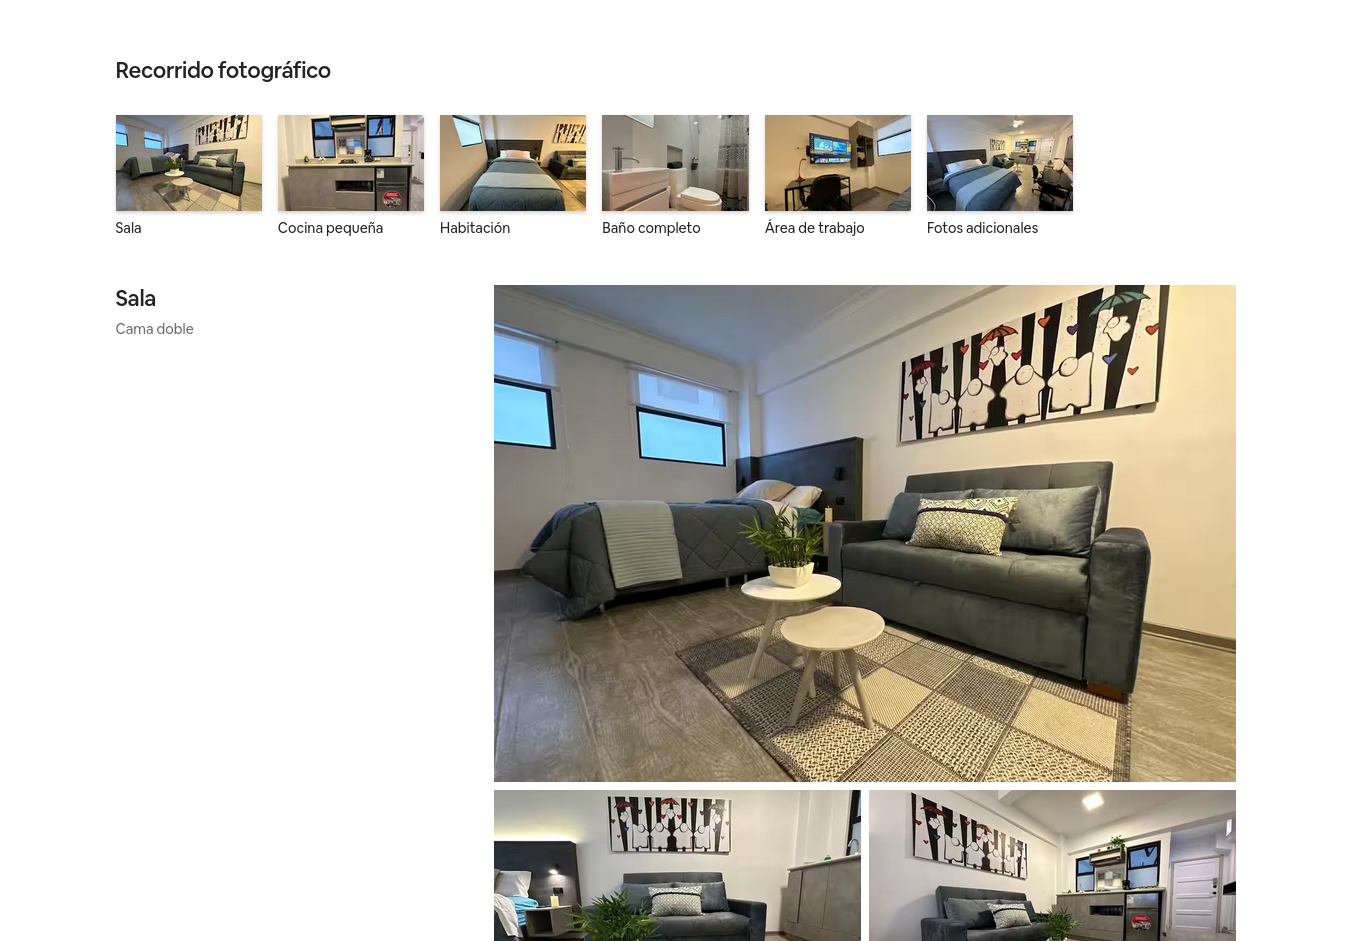
\includegraphics[height=0.50\textheight,width=0.96\linewidth,keepaspectratio,trim=65 35 65 45,clip]{../references/airbnb_recom.png}}

\vspace{0.12cm}
{\color{gray} Fotos etiquetadas autom\'aticamente:}\\[-1pt]
{\color{green!60!black}\textbf{Sala} $\cdot$ \textbf{Cocina} $\cdot$ \textbf{Habitaci\'on} $\cdot$ \textbf{Ba\~no}}
\end{column}

\begin{column}{0.49\textwidth}
\centering
{\large\textbf{\color{red!60!black}Urbania.pe --- Sin clasificaci\'on}}

\vspace{0.12cm}
\setlength{\fboxsep}{2pt}
\fcolorbox{red!55!black}{white}{%
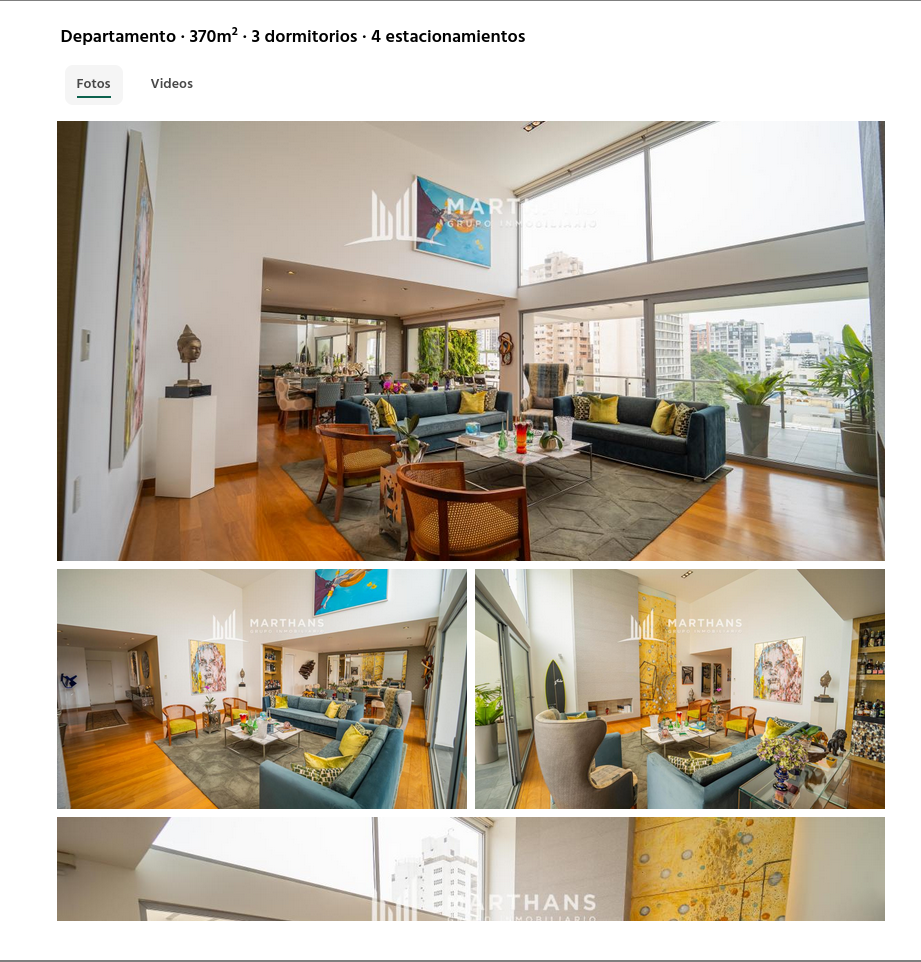
\includegraphics[height=0.50\textheight,width=0.96\linewidth,keepaspectratio,trim=35 35 35 35,clip]{../references/urbania_no_recom.png}}

\vspace{0.12cm}
{\color{gray} Solo carrusel de fotos:}\\[-1pt]
{\color{red!60!black}\textbf{Sin etiquetas} $\cdot$ \textbf{Sin categorizaci\'on} $\cdot$ \textbf{Ca\'otico}}
\end{column}
\end{columns}

\vspace{0.18cm}
\centering
\begin{beamercolorbox}[rounded=true,sep=0.06cm,center,wd=0.86\textwidth]{block body}
\textbf{Oportunidad:} convertir carruseles sin estructura en recorridos fotogr\'aficos categorizados.
\end{beamercolorbox}
\end{frame}

\begin{frame}{Qu\'e aporta este trabajo}
\begin{enumerate}
\item Dataset y pipeline reproducible desde Urbania.pe: scraping, auto-etiquetado y curaci\'on manual
\item Comparaci\'on sistem\'atica: CLIP zero-shot vs embeddings CLIP/DINOv2/Place365 + clasificadores ML
\item Dise\~no experimental con split antes del aumento para evitar fuga de datos
\item Prototipo Streamlit con tres modos de uso para llevar el modelo a una demo operativa
\end{enumerate}
\end{frame}

\section{Metodolog\'ia}

\begin{frame}[plain]
\centering
\resizebox{0.96\paperwidth}{!}{%
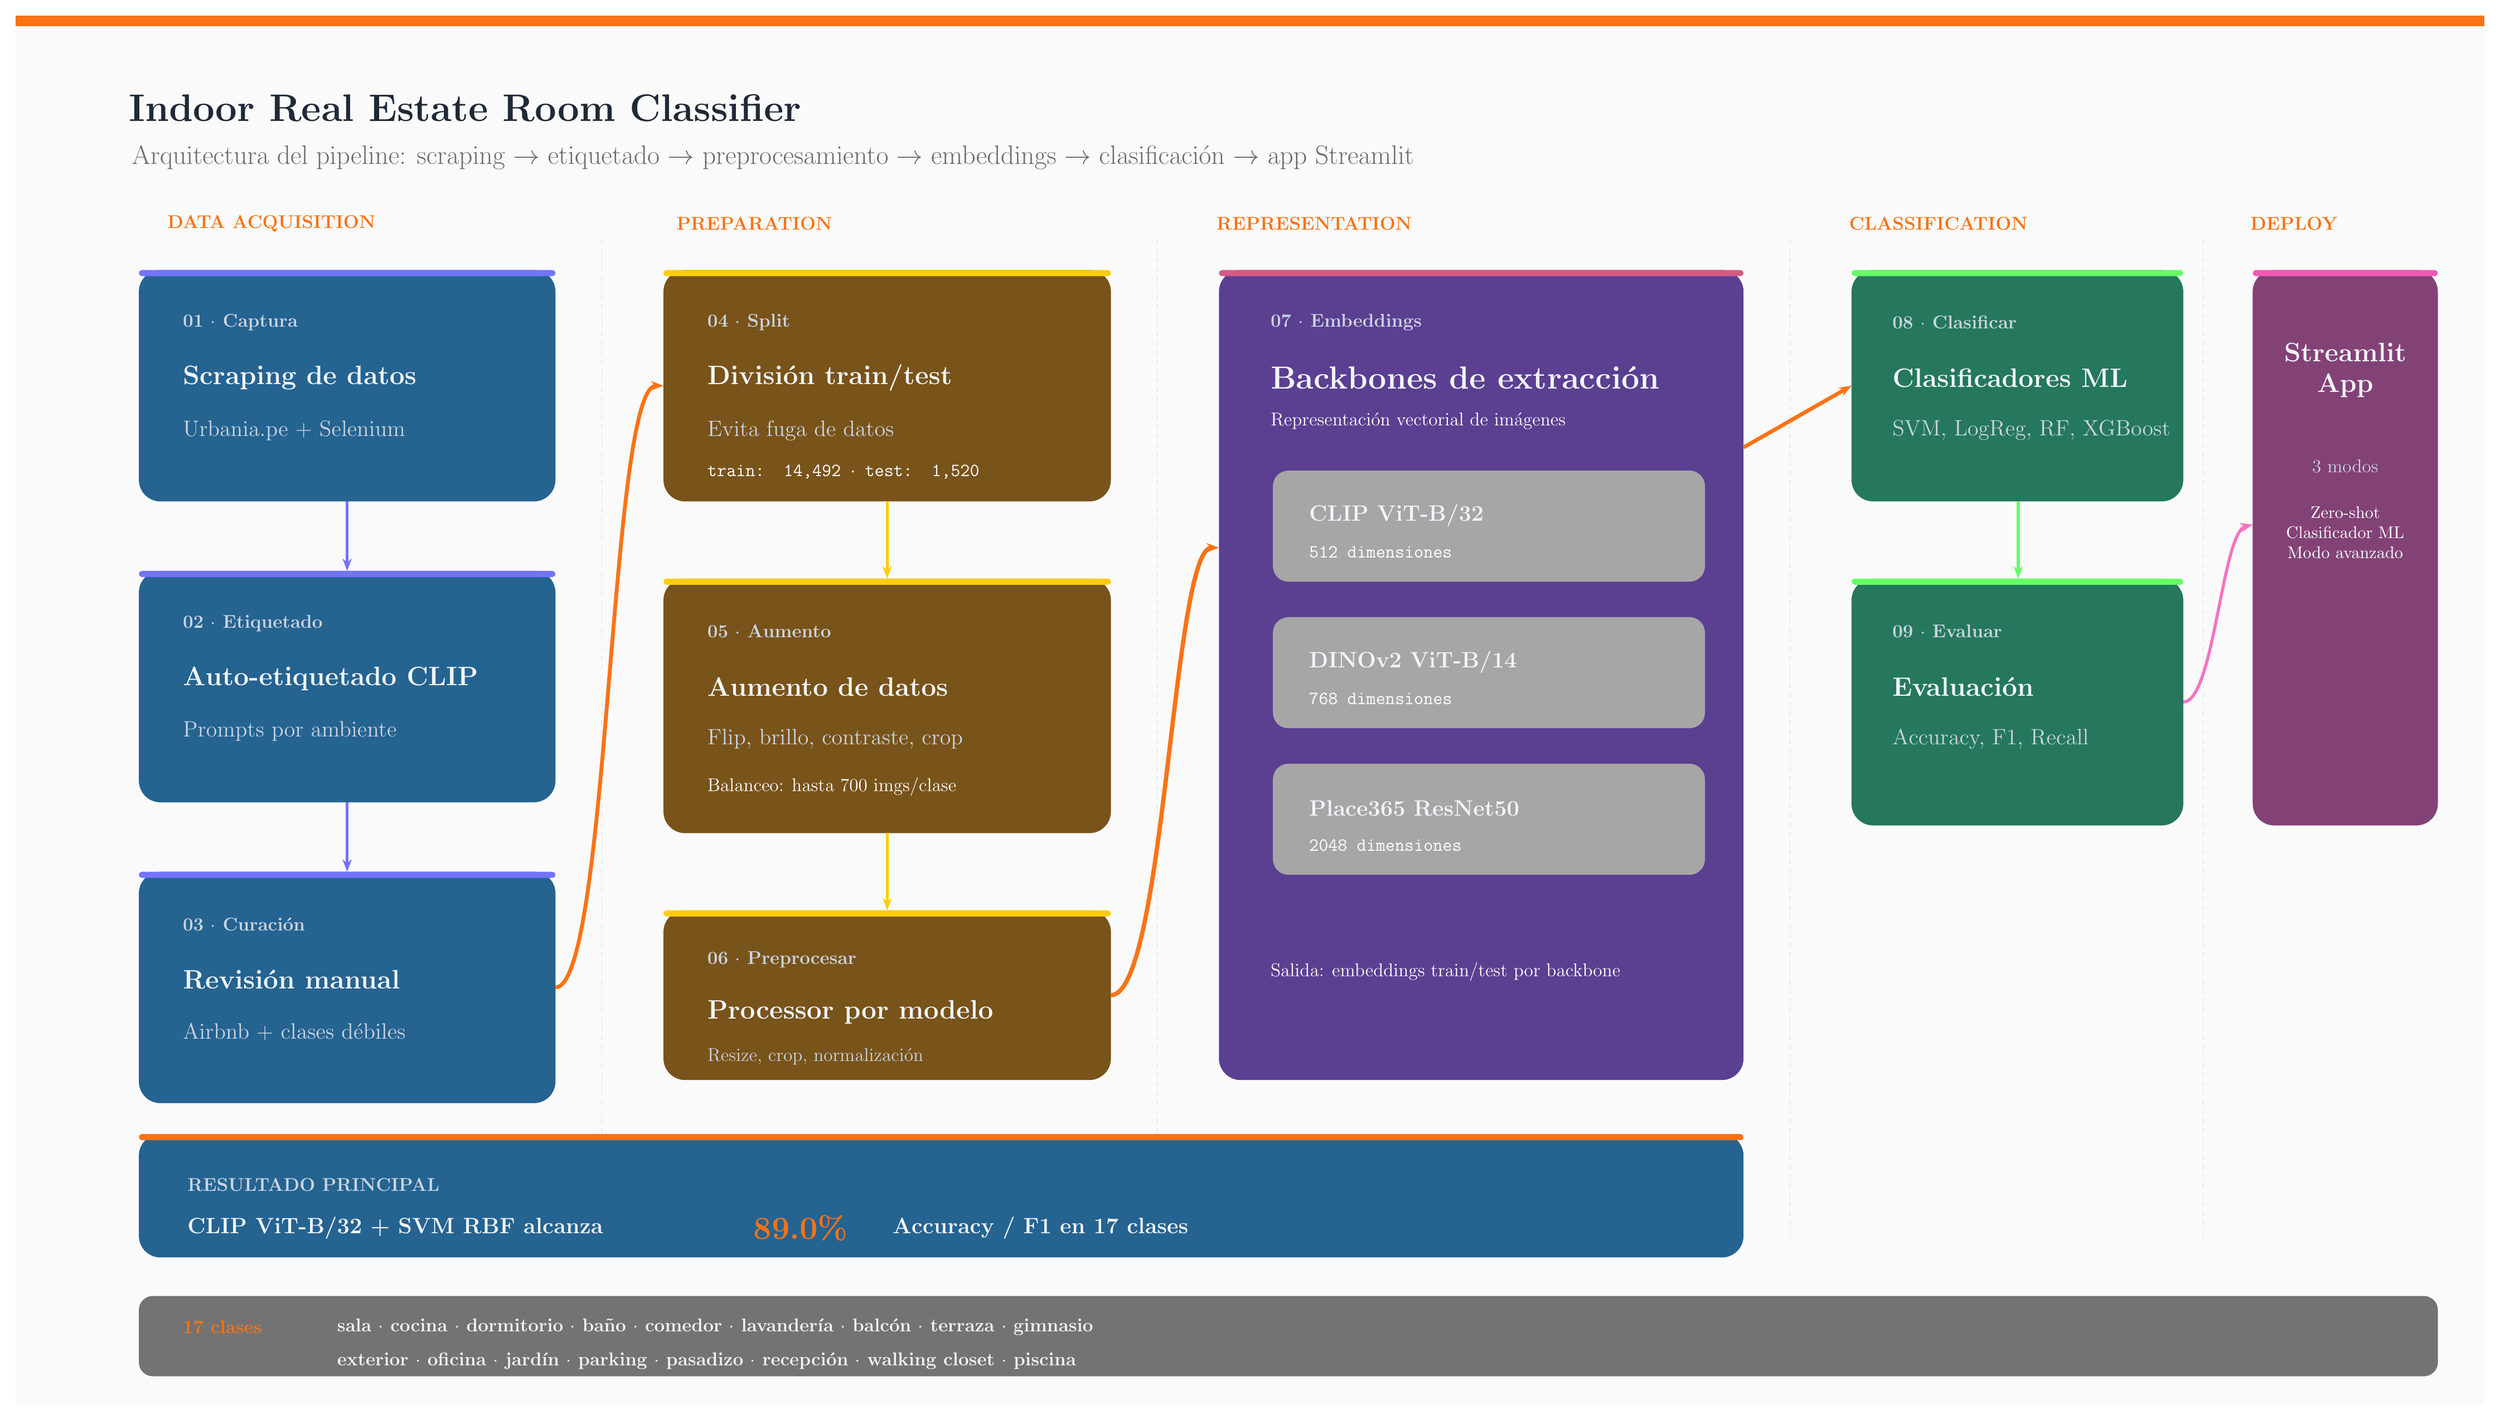
\begin{tikzpicture}[x=1pt,y=-1pt]
  \path[use as bounding box] (0,0) rectangle (1600,900);
  \fill[gray!4] (0,0) rectangle (1600,900);
  \fill[accentorange] (0,0) rectangle (1600,7);

  \node[anchor=west, text=nightbg, font=\bfseries\fontsize{34}{38}\selectfont] at (70,60) {Indoor Real Estate Room Classifier};
  \node[anchor=west, text=black!58, font=\fontsize{16}{18}\selectfont] at (72,92) {Arquitectura del pipeline: scraping $\rightarrow$ etiquetado $\rightarrow$ preprocesamiento $\rightarrow$ embeddings $\rightarrow$ clasificaci\'on $\rightarrow$ app Streamlit};

  \node[anchor=west, text=accentorange, font=\bfseries\fontsize{12}{14}\selectfont] at (95,135) {DATA ACQUISITION};
  \node[anchor=west, text=accentorange, font=\bfseries\fontsize{12}{14}\selectfont] at (425,135) {PREPARATION};
  \node[anchor=west, text=accentorange, font=\bfseries\fontsize{12}{14}\selectfont] at (775,135) {REPRESENTATION};
  \node[anchor=west, text=accentorange, font=\bfseries\fontsize{12}{14}\selectfont] at (1185,135) {CLASSIFICATION};
  \node[anchor=west, text=accentorange, font=\bfseries\fontsize{12}{14}\selectfont] at (1445,135) {DEPLOY};
  \draw[dashed, color=black!14] (380,145) -- (380,795);
  \draw[dashed, color=black!14] (740,145) -- (740,795);
  \draw[dashed, color=black!14] (1150,145) -- (1150,795);
  \draw[dashed, color=black!14] (1418,145) -- (1418,795);

  % Data cards
  \foreach \y/\n/\t/\a/\b in {165/01/Captura/Scraping de datos/Urbania.pe + Selenium,360/02/Etiquetado/Auto-etiquetado CLIP/Prompts por ambiente,555/03/Curaci\'on/Revisi\'on manual/Airbnb + clases d\'ebiles} {
    \fill[carddata, rounded corners=14pt] (80,\y) rectangle (350,{\y+150});
    \fill[blue!55, rounded corners=2pt] (80,\y) rectangle (350,{\y+4});
    \node[anchor=west, text=textmuted, font=\bfseries\fontsize{12}{14}\selectfont] at (105,{\y+34}) {\n\ $\cdot$ \t};
    \node[anchor=west, text=textlight, font=\bfseries\fontsize{19}{22}\selectfont] at (105,{\y+70}) {\a};
    \node[anchor=west, text=textmuted, font=\fontsize{14}{16}\selectfont] at (105,{\y+104}) {\b};
  }

  % Prep cards
  \fill[cardprep, rounded corners=14pt] (420,165) rectangle (710,315);
  \fill[yellow!65!orange, rounded corners=2pt] (420,165) rectangle (710,169);
  \node[anchor=west, text=textmuted, font=\bfseries\fontsize{12}{14}\selectfont] at (445,199) {04 $\cdot$ Split};
  \node[anchor=west, text=textlight, font=\bfseries\fontsize{19}{22}\selectfont] at (445,235) {Divisi\'on train/test};
  \node[anchor=west, text=textmuted, font=\fontsize{14}{16}\selectfont] at (445,269) {Evita fuga de datos};
  \node[anchor=west, text=white!45, font=\ttfamily\fontsize{12}{14}\selectfont] at (445,296) {train: 14,492 $\cdot$ test: 1,520};

  \fill[cardprep, rounded corners=14pt] (420,365) rectangle (710,530);
  \fill[yellow!65!orange, rounded corners=2pt] (420,365) rectangle (710,369);
  \node[anchor=west, text=textmuted, font=\bfseries\fontsize{12}{14}\selectfont] at (445,399) {05 $\cdot$ Aumento};
  \node[anchor=west, text=textlight, font=\bfseries\fontsize{19}{22}\selectfont] at (445,435) {Aumento de datos};
  \node[anchor=west, text=textmuted, font=\fontsize{14}{16}\selectfont] at (445,469) {Flip, brillo, contraste, crop};
  \node[anchor=west, text=white!45, font=\fontsize{12}{14}\selectfont] at (445,500) {Balanceo: hasta 700 imgs/clase};

  \fill[cardprep, rounded corners=14pt] (420,580) rectangle (710,690);
  \fill[yellow!65!orange, rounded corners=2pt] (420,580) rectangle (710,584);
  \node[anchor=west, text=textmuted, font=\bfseries\fontsize{12}{14}\selectfont] at (445,612) {06 $\cdot$ Preprocesar};
  \node[anchor=west, text=textlight, font=\bfseries\fontsize{18}{21}\selectfont] at (445,646) {Processor por modelo};
  \node[anchor=west, text=textmuted, font=\fontsize{13}{15}\selectfont] at (445,675) {Resize, crop, normalizaci\'on};

  % Embeddings card
  \fill[cardembed, rounded corners=14pt] (780,165) rectangle (1120,690);
  \fill[purple!65, rounded corners=2pt] (780,165) rectangle (1120,169);
  \node[anchor=west, text=textmuted, font=\bfseries\fontsize{12}{14}\selectfont] at (810,199) {07 $\cdot$ Embeddings};
  \node[anchor=west, text=textlight, font=\bfseries\fontsize{20}{23}\selectfont] at (810,235) {Backbones de extracci\'on};
  \node[anchor=west, text=white!45, font=\fontsize{13}{15}\selectfont] at (810,263) {Representaci\'on vectorial de im\'agenes};
  \fill[black!35, rounded corners=10pt] (815,295) rectangle (1095,367);
  \node[anchor=west, text=textlight, font=\bfseries\fontsize{15}{17}\selectfont] at (835,324) {CLIP ViT-B/32};
  \node[anchor=west, text=white!70, font=\ttfamily\fontsize{12}{14}\selectfont] at (835,348) {512 dimensiones};
  \fill[black!35, rounded corners=10pt] (815,390) rectangle (1095,462);
  \node[anchor=west, text=textlight, font=\bfseries\fontsize{15}{17}\selectfont] at (835,419) {DINOv2 ViT-B/14};
  \node[anchor=west, text=white!70, font=\ttfamily\fontsize{12}{14}\selectfont] at (835,443) {768 dimensiones};
  \fill[black!35, rounded corners=10pt] (815,485) rectangle (1095,557);
  \node[anchor=west, text=textlight, font=\bfseries\fontsize{15}{17}\selectfont] at (835,514) {Place365 ResNet50};
  \node[anchor=west, text=white!70, font=\ttfamily\fontsize{12}{14}\selectfont] at (835,538) {2048 dimensiones};
  \node[anchor=west, text=white!45, font=\fontsize{13}{15}\selectfont] at (810,620) {Salida: embeddings train/test por backbone};

  % Classifier and evaluation
  \fill[cardclf, rounded corners=14pt] (1190,165) rectangle (1405,315);
  \fill[green!60, rounded corners=2pt] (1190,165) rectangle (1405,169);
  \node[anchor=west, text=textmuted, font=\bfseries\fontsize{12}{14}\selectfont] at (1213,199) {08 $\cdot$ Clasificar};
  \node[anchor=west, text=textlight, font=\bfseries\fontsize{19}{22}\selectfont] at (1213,235) {Clasificadores ML};
  \node[anchor=west, text=textmuted, font=\fontsize{14}{16}\selectfont] at (1213,269) {SVM, LogReg, RF, XGBoost};

  \fill[cardclf, rounded corners=14pt] (1190,365) rectangle (1405,525);
  \fill[green!60, rounded corners=2pt] (1190,365) rectangle (1405,369);
  \node[anchor=west, text=textmuted, font=\bfseries\fontsize{12}{14}\selectfont] at (1213,399) {09 $\cdot$ Evaluar};
  \node[anchor=west, text=textlight, font=\bfseries\fontsize{19}{22}\selectfont] at (1213,435) {Evaluaci\'on};
  \node[anchor=west, text=textmuted, font=\fontsize{14}{16}\selectfont] at (1213,469) {Accuracy, F1, Recall};

  \fill[cardapp, rounded corners=14pt] (1450,165) rectangle (1570,525);
  \fill[magenta!65, rounded corners=2pt] (1450,165) rectangle (1570,169);
  \node[text=textlight, font=\bfseries\fontsize{17}{20}\selectfont, align=center] at (1510,230) {Streamlit\\App};
  \node[text=textmuted, font=\fontsize{12}{14}\selectfont, align=center] at (1510,292) {3 modos};
  \node[text=white!65, font=\fontsize{11}{13}\selectfont, align=center] at (1510,335) {Zero-shot\\Clasificador ML\\Modo avanzado};

  % Result card
  \fill[carddata, rounded corners=14pt] (80,725) rectangle (1120,805);
  \fill[accentorange, rounded corners=2pt] (80,725) rectangle (1120,729);
  \node[anchor=west, text=textmuted, font=\bfseries\fontsize{12}{14}\selectfont] at (108,758) {RESULTADO PRINCIPAL};
  \node[anchor=west, text=textlight, font=\bfseries\fontsize{15}{18}\selectfont] at (108,786) {CLIP ViT-B/32 + SVM RBF alcanza};
  \node[anchor=west, text=accentorange, font=\bfseries\fontsize{22}{25}\selectfont] at (475,786) {89.0\%};
  \node[anchor=west, text=textlight, font=\bfseries\fontsize{15}{18}\selectfont] at (565,786) {Accuracy / F1 en 17 clases};

  % Classes footer
  \fill[black!55, rounded corners=9pt] (80,830) rectangle (1570,882);
  \node[anchor=west, text=accentorange, font=\bfseries\fontsize{12}{14}\selectfont] at (105,850) {17 clases};
  \node[anchor=west, text=textlight, font=\bfseries\fontsize{12}{14}\selectfont] at (205,850) {sala $\cdot$ cocina $\cdot$ dormitorio $\cdot$ ba\~no $\cdot$ comedor $\cdot$ lavander\'ia $\cdot$ balc\'on $\cdot$ terraza $\cdot$ gimnasio};
  \node[anchor=west, text=textlight, font=\bfseries\fontsize{12}{14}\selectfont] at (205,872) {exterior $\cdot$ oficina $\cdot$ jard\'in $\cdot$ parking $\cdot$ pasadizo $\cdot$ recepci\'on $\cdot$ walking closet $\cdot$ piscina};

  % Arrows
  \draw[-{Stealth[length=8pt,width=6pt]}, line width=2pt, color=blue!55] (215,315) -- (215,360);
  \draw[-{Stealth[length=8pt,width=6pt]}, line width=2pt, color=blue!55] (215,510) -- (215,555);
  \draw[-{Stealth[length=8pt,width=6pt]}, line width=2.5pt, color=accentorange] (350,630) .. controls (385,630) and (385,240) .. (420,240);
  \draw[-{Stealth[length=8pt,width=6pt]}, line width=2pt, color=yellow!65!orange] (565,315) -- (565,365);
  \draw[-{Stealth[length=8pt,width=6pt]}, line width=2pt, color=yellow!65!orange] (565,530) -- (565,580);
  \draw[-{Stealth[length=8pt,width=6pt]}, line width=2.8pt, color=accentorange] (710,635) .. controls (745,635) and (750,345) .. (780,345);
  \draw[-{Stealth[length=8pt,width=6pt]}, line width=2.5pt, color=accentorange] (1120,280) -- (1190,240);
  \draw[-{Stealth[length=8pt,width=6pt]}, line width=2pt, color=green!60] (1298,315) -- (1298,365);
  \draw[-{Stealth[length=8pt,width=6pt]}, line width=2pt, color=magenta!55] (1405,445) .. controls (1425,445) and (1430,335) .. (1450,330);
\end{tikzpicture}%
}
\end{frame}

\begin{frame}{Extracci\'on de Caracter\'isticas: Del Baseline a Foundation Models}
\footnotesize
\begin{columns}
\begin{column}{0.48\textwidth}
\textbf{Baseline: Place365 ResNet50}\\
(MIT CSAIL)
\begin{itemize}
\item Pre-entrenado en MIT Indoor Scenes (365 categor\'ias)
\item 1.8M im\'agenes de escenas indoor/outdoor
\item CNN (no transformer), 2048 dimensiones
\end{itemize}
{\scriptsize\color{gray} Ref.: Zhou et al., \textit{Places: A 10 Million Image Database for Scene Recognition}, TPAMI 2017.}

\vspace{0.15cm}
\textbf{CLIP ViT-B/32} (OpenAI)
\begin{itemize}
\item Im\'agenes + texto $\rightarrow$ espacio compartido
\item 512 dimensiones, alineado con lenguaje
\item Entrenado en WIT (400M pares)
\end{itemize}

\vspace{0.15cm}
\textbf{DINOv2 ViT-B/14} (Meta)
\begin{itemize}
\item Auto-supervisado en LVD-142M
\item 768 dimensiones, sin lenguaje
\end{itemize}
\end{column}

\begin{column}{0.48\textwidth}
\textbf{Embeddings extra\'idos}
\begin{table}
\centering
\scriptsize
\begin{tabular}{@{}lcc@{}}
\toprule
\textbf{Backbone} & \textbf{Dim} & \textbf{Total} \\
\midrule
CLIP ViT-B/32 & 512 & 16,012 \\
DINOv2 ViT-B/14 & 768 & 16,012 \\
Place365 ResNet50 & 2048 & 16,012 \\
\bottomrule
\end{tabular}
\end{table}

\vspace{0.15cm}
\footnotesize 14,492 train + 1,520 test\\
L2-normalizados y cacheados a disco

\vspace{0.15cm}
\textbf{Clasificadores:}
\begin{itemize}
\item SVM RBF (mejor para CLIP y DINOv2)
\item XGBoost (mejor para Place365)
\end{itemize}
\end{column}
\end{columns}
\end{frame}

\begin{frame}{Preprocesamiento: Comparaci\'on Justa entre Backbones}
\footnotesize
\centering
{\small Antes de comparar CLIP, DINOv2 y Place365, cada imagen debe entrar al modelo como ese modelo espera verla.}

\vspace{0.08cm}
\begin{table}
\centering
\scriptsize
\begin{tabular}{@{}llccc@{}}
\toprule
\textbf{Modelo} & \textbf{Dataset base} & \textbf{Fuente del preproc.} & \textbf{Res.} & \textbf{Norm.} \\
\midrule
CLIP & WIT (400M pares) & CLIPProcessor oficial & 224$\times$224 & Stats WIT \\
DINOv2 & LVD-142M & AutoImageProcessor oficial & 224$\times$224 & ImageNet \\
Place365 & MIT Indoor Scenes & Receta Places365/torchvision & 224$\times$224 & ImageNet \\
\bottomrule
\end{tabular}
\end{table}

\vspace{0.08cm}
\begin{columns}[T,totalwidth=\textwidth]
\begin{column}{0.48\textwidth}
\textbf{Misma imagen, tres entradas}
\begin{itemize}
\item CLIP usa su \textit{processor} oficial
\item DINOv2 usa su \textit{AutoImageProcessor}
\item Place365 sigue la receta de escenas indoor
\end{itemize}
\end{column}

\begin{column}{0.48\textwidth}
\textbf{Salida comparable}
\begin{itemize}
\item Todas producen tensor (1, 3, 224, 224)
\item Se extraen embeddings para train y test
\item 16,012 embeddings por backbone
\end{itemize}
\end{column}
\end{columns}
\end{frame}

\begin{frame}{Aumento de Datos: M\'as Datos sin Enga\~nar al Test}
\footnotesize
\begin{columns}[T,totalwidth=\textwidth]
\begin{column}{0.52\textwidth}
\textbf{El problema}\
Algunas clases ten\'ian pocas im\'agenes y alta variabilidad visual: balcones, terrazas, pasadizos o \textit{walking closets}.

\vspace{0.18cm}
\textbf{El riesgo}\
Si se aumenta antes de separar train/test, una versi\'on casi duplicada de una imagen puede aparecer en ambos conjuntos.

\vspace{0.18cm}
\begin{beamercolorbox}[rounded=true,sep=0.08cm,wd=\linewidth]{block body}
\textbf{Decisi\'on experimental:} primero split, despu\'es aumento solo en train.
\end{beamercolorbox}

\vspace{0.12cm}
\begin{itemize}
\item Test intacto: 1,520 im\'agenes reales, sin transformaciones
\item Train balanceado hasta 700 im\'agenes por clase
\item Objetivo: robustez en clases minoritarias, no inflar la m\'etrica
\end{itemize}
\end{column}

\begin{column}{0.45\textwidth}
\textbf{Transformaciones realistas}
\begin{table}
\centering
\scriptsize
\begin{tabular}{@{}ll@{}}
\toprule
\textbf{Transformaci\'on} & \textbf{Intenci\'on} \\
\midrule
Crop leve & Encuadres distintos \\
Flip horizontal & Simetr\'ia de ambientes \\
Brillo/contraste & Condiciones de luz \\
Rotaci\'on $\pm$5$^\circ$ & Fotos torcidas \\
Perspectiva suave & Toma desde celular \\
Blur/JPEG & Calidad de anuncio \\
\bottomrule
\end{tabular}
\end{table}

\vspace{0.12cm}
\textbf{Lo que se evit\'o}
\begin{itemize}
\item Rotaciones 90$^\circ$/180$^\circ$ y vertical flip
\item Recortes extremos, MixUp y CutMix
\item Cambios de color agresivos
\end{itemize}
\end{column}
\end{columns}

\vspace{0.12cm}
\centering
{\small La mejora buscada no era crear im\'agenes nuevas, sino ense\~nar invariancias que aparecen en anuncios inmobiliarios reales.}
\end{frame}

\section{Resultados}

\begin{frame}{Comparaci\'on de Modelos}
\begin{table}
\centering
\small
\begin{tabular}{@{}llcccc@{}}
\toprule
\textbf{Backbone} & \textbf{Dataset} & \textbf{Acc.} & \textbf{F1} & \textbf{Prec.} & \textbf{Rec.} \\
\midrule
\textbf{CLIP + SVM} & WIT & \textbf{89.0\%} & \textbf{89.0\%} & \textbf{89.1\%} & \textbf{89.0\%} \\
DINOv2 + SVM & LVD-142M & 88.3\% & 88.4\% & 88.7\% & 88.3\% \\
Place365 + XGB & MIT Indoor & 86.2\% & 86.2\% & 86.4\% & 86.2\% \\
\midrule
CLIP Zero-shot & WIT & 72.2\% & 75.2\% & 84.9\% & 72.2\% \\
\bottomrule
\end{tabular}
\vspace{0.12cm}

{\footnotesize Test: 1,520 im\'agenes, 17 clases $\cdot$ 16,012 embeddings por backbone (14,492 train + 1,520 test)}
\end{table}
\end{frame}

\begin{frame}{CLIP Zero-shot vs CLIP + SVM Classifier}
\footnotesize
\begin{columns}[T,totalwidth=\textwidth]
\begin{column}{0.49\textwidth}
\centering
{\large\textbf{CLIP Zero-shot}}\\[-1pt]
{\scriptsize Modelo CLIP por defecto, sin entrenamiento supervisado}

\vspace{0.04cm}
\setlength{\fboxsep}{1pt}
\fcolorbox{gray!35}{white}{%
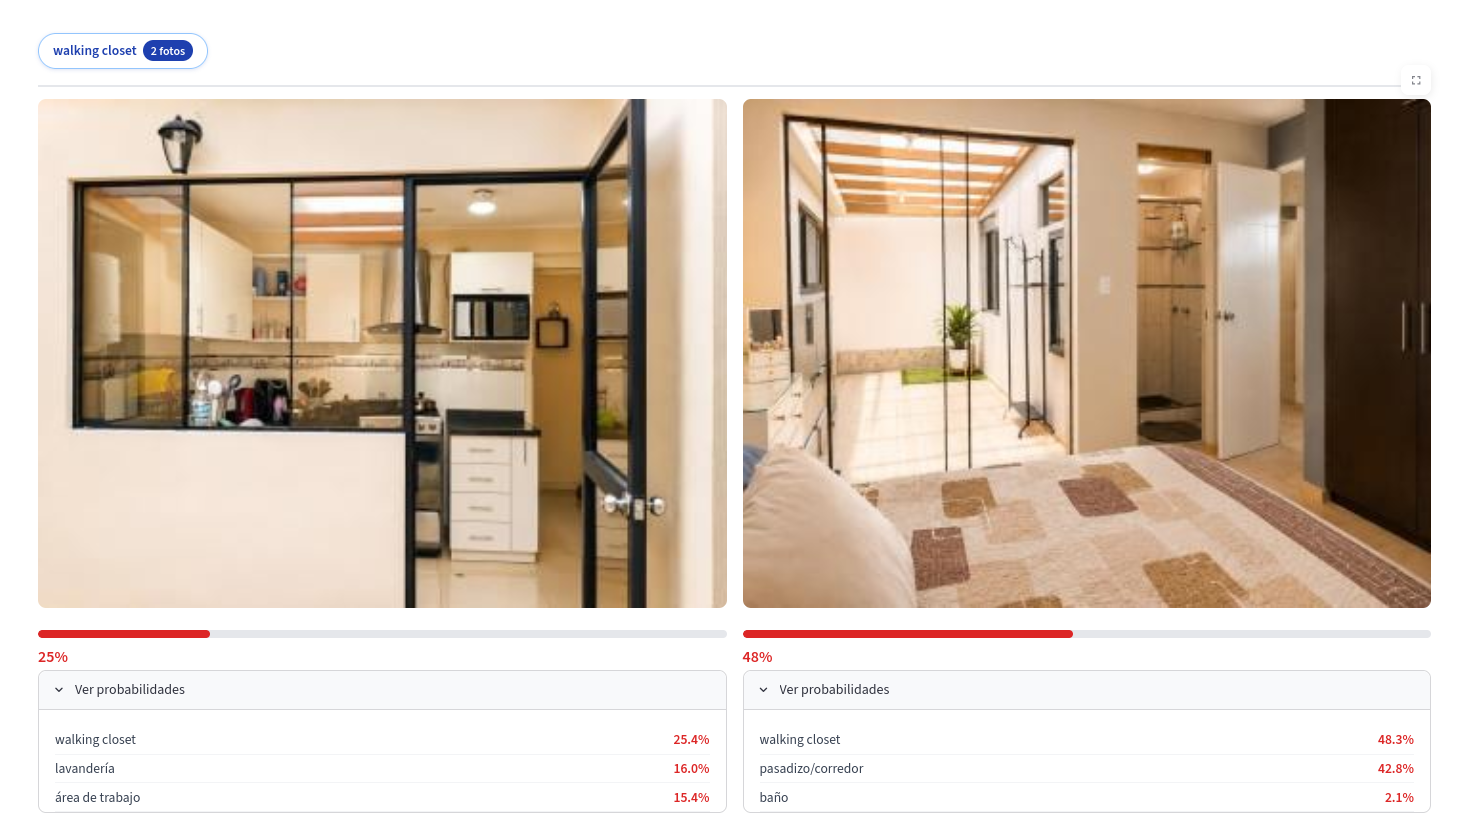
\includegraphics[width=\linewidth,height=0.37\textheight,keepaspectratio]{../references/zero_shot_clip.png}}

\vspace{0.06cm}
\begin{beamercolorbox}[rounded=true,sep=0.05cm,center,wd=0.82\linewidth]{block body}
\scriptsize Predice como \textbf{Walking Closet}
\end{beamercolorbox}
\end{column}

\begin{column}{0.49\textwidth}
\centering
{\large\textbf{CLIP + SVM Classifier}}\\[-1pt]
{\scriptsize Embeddings CLIP congelados + SVM RBF entrenado}

\vspace{0.04cm}
\setlength{\fboxsep}{1pt}
\fcolorbox{gray!35}{white}{%
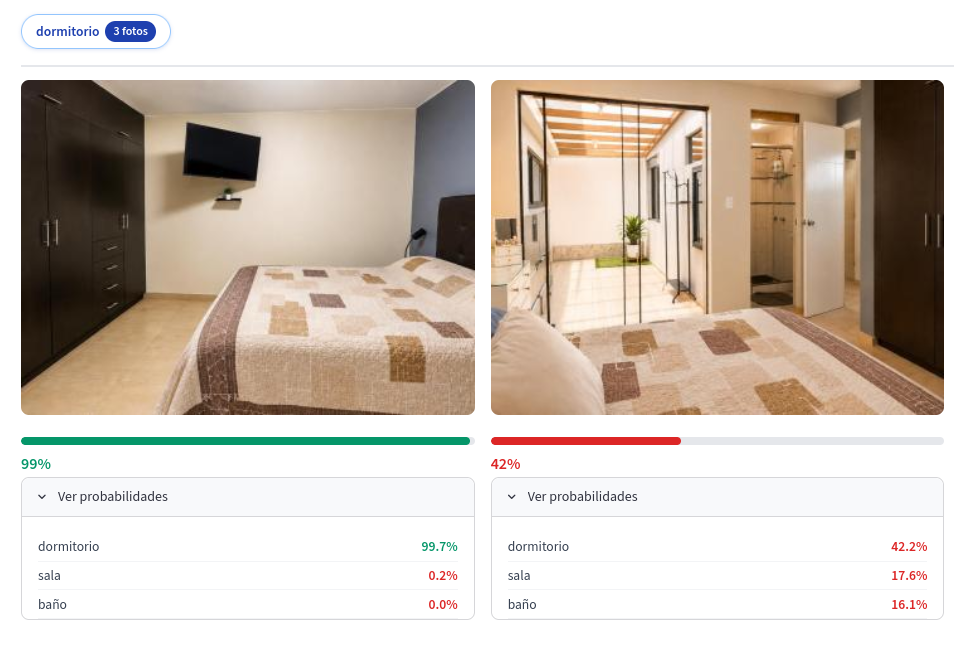
\includegraphics[width=\linewidth,height=0.37\textheight,keepaspectratio]{../references/clip_svm.png}}

\vspace{0.06cm}
\begin{beamercolorbox}[rounded=true,sep=0.05cm,center,wd=0.82\linewidth]{block body}
\scriptsize Predice como \textbf{Dormitorio}
\end{beamercolorbox}
\end{column}
\end{columns}

\vspace{0.08cm}
\centering
\begin{beamercolorbox}[rounded=true,sep=0.05cm,center,wd=0.88\textwidth]{block body}
\scriptsize
Mismo backbone visual (CLIP), pero el SVM aprende la frontera entre las 17 clases del dominio inmobiliario: +13.8 puntos F1 frente al zero-shot.
\end{beamercolorbox}
\end{frame}

\begin{frame}{Hallazgos Clave}
\begin{enumerate}
\item \textbf{CLIP $\approx$ DINOv2 > Place365} -- 89.0\% vs 88.4\% vs 86.2\% F1
\item \textbf{SVM RBF} convierte embeddings congelados en un clasificador competitivo
\item \textbf{CLIP zero-shot} es una base razonable, pero queda 14 puntos F1 por debajo del SVM
\item \textbf{Aumento de datos} mejora +3.1\% F1 cuando se aplica solo al train
\end{enumerate}

\vspace{0.5cm}
\textbf{Lectura principal:} no hace falta fine-tunear un modelo grande; extraer buenas representaciones y entrenar un clasificador liviano alcanza 89.0\% F1.
\end{frame}

\begin{frame}{Rendimiento por Clase: D\'onde el Modelo es Confiable}
\footnotesize
\centering
{\small El 89.0\% global no se distribuye igual: algunas clases son visualmente claras y otras viven en zonas grises.}

\vspace{0.16cm}
\begin{columns}[T,totalwidth=\textwidth]
\begin{column}{0.31\textwidth}
\begin{beamercolorbox}[rounded=true,sep=0.12cm,wd=\linewidth]{block body}
\centering
\textbf{Muy confiables}\\[-1pt]
\scriptsize F1 $\geq$ 0.93
\end{beamercolorbox}
\vspace{0.08cm}
\begin{itemize}
\item Gimnasio: \textbf{1.000}
\item Ba\~no: \textbf{0.949}
\item Cocina: \textbf{0.945}
\item Piscina: \textbf{0.932}
\end{itemize}
\vspace{0.05cm}
{\scriptsize Rasgos visuales distintivos: equipamiento, superficies y objetos espec\'ificos.}
\end{column}

\begin{column}{0.33\textwidth}
\begin{beamercolorbox}[rounded=true,sep=0.12cm,wd=\linewidth]{block body}
\centering
\textbf{Robustas, pero variables}\\[-1pt]
\scriptsize F1 $\approx$ 0.89--0.90
\end{beamercolorbox}
\vspace{0.08cm}
\begin{itemize}
\item Sala: \textbf{0.901}
\item Dormitorio: \textbf{0.897}
\item Walking Closet: \textbf{0.889}
\item Pasadizo: \textbf{0.889}
\end{itemize}
\vspace{0.05cm}
{\scriptsize Funcionan bien, aunque cambian mucho por estilo, encuadre y tama\~no del ambiente.}
\end{column}

\begin{column}{0.31\textwidth}
\begin{beamercolorbox}[rounded=true,sep=0.12cm,wd=\linewidth]{block body}
\centering
\textbf{Zonas grises}\\[-1pt]
\scriptsize F1 $<$ 0.77
\end{beamercolorbox}
\vspace{0.08cm}
\begin{itemize}
\item Terraza: \textbf{0.763}
\item Balc\'on: \textbf{0.750}
\item Patio/Jard\'in: \textbf{0.722}
\item \'Area de trabajo: \textbf{0.667}
\end{itemize}
\vspace{0.05cm}
{\scriptsize Comparten objetos, luz y distribuci\'on espacial con exterior, sala u oficina.}
\end{column}
\end{columns}

\end{frame}

\begin{frame}{F1 por Clase y Modelo}
\centering
\scriptsize
\begin{columns}[T]
\begin{column}{0.49\textwidth}
\begin{tabular}{@{}lcccc@{}}
\toprule
\textbf{Clase} & \textbf{CLIP} & \textbf{DINO} & \textbf{Place} & \textbf{Mejor} \\
\midrule
gimnasio & \textbf{1.000} & \textbf{1.000} & 0.962 & empate \\
ba\~no & \textbf{0.949} & 0.933 & 0.898 & CLIP \\
cocina & \textbf{0.945} & 0.924 & 0.931 & CLIP \\
piscina & \textbf{0.932} & 0.913 & 0.902 & CLIP \\
dormitorio & 0.897 & \textbf{0.923} & 0.884 & DINO \\
sala & \textbf{0.901} & 0.892 & 0.888 & CLIP \\
walking closet & 0.889 & \textbf{0.919} & 0.850 & DINO \\
pasadizo & 0.889 & \textbf{0.910} & 0.865 & DINO \\
exterior & \textbf{0.873} & 0.865 & 0.817 & CLIP \\
\bottomrule
\end{tabular}
\end{column}
\begin{column}{0.49\textwidth}
\begin{tabular}{@{}lcccc@{}}
\toprule
\textbf{Clase} & \textbf{CLIP} & \textbf{DINO} & \textbf{Place} & \textbf{Mejor} \\
\midrule
comedor & \textbf{0.866} & 0.845 & 0.844 & CLIP \\
lavander\'ia & 0.857 & 0.857 & \textbf{0.870} & Place \\
estacionamiento & 0.833 & \textbf{0.917} & 0.889 & DINO \\
recepci\'on & 0.815 & \textbf{0.880} & 0.667 & DINO \\
terraza & \textbf{0.763} & 0.636 & 0.658 & CLIP \\
balc\'on & 0.750 & \textbf{0.764} & 0.727 & DINO \\
patio/jard\'in & \textbf{0.722} & 0.709 & 0.624 & CLIP \\
\'area trabajo & \textbf{0.667} & 0.606 & 0.429 & CLIP \\
\midrule
\textbf{Victorias} & \textbf{10} & \textbf{6} & \textbf{1} & \\
\bottomrule
\end{tabular}
\end{column}
\end{columns}

\vspace{0.2cm}
{\footnotesize CLIP gana en 10/17 clases; DINOv2 destaca en clases estrechas o con bajo soporte; Place365 solo gana en lavander\'ia.}
\end{frame}

\section{Demo}

\begin{frame}{Del mejor modelo a una demo navegable}
\begin{columns}[T,totalwidth=\textwidth]
\begin{column}{0.34\textwidth}
\footnotesize
\begin{itemize}
\item Subida de im\'agenes de una propiedad
\item Agrupaci\'on autom\'atica por ambiente
\item Comparaci\'on entre zero-shot, clasificador ML y modo avanzado
\item Mejora extra: detecci\'on YOLO11n de muebles/objetos indoor con datasets Roboflow
\item Salida pensada para ordenar carruseles inmobiliarios
\end{itemize}

\end{column}

\begin{column}{0.64\textwidth}
\centering
\setlength{\fboxsep}{1pt}
\fcolorbox{gray!35}{white}{%
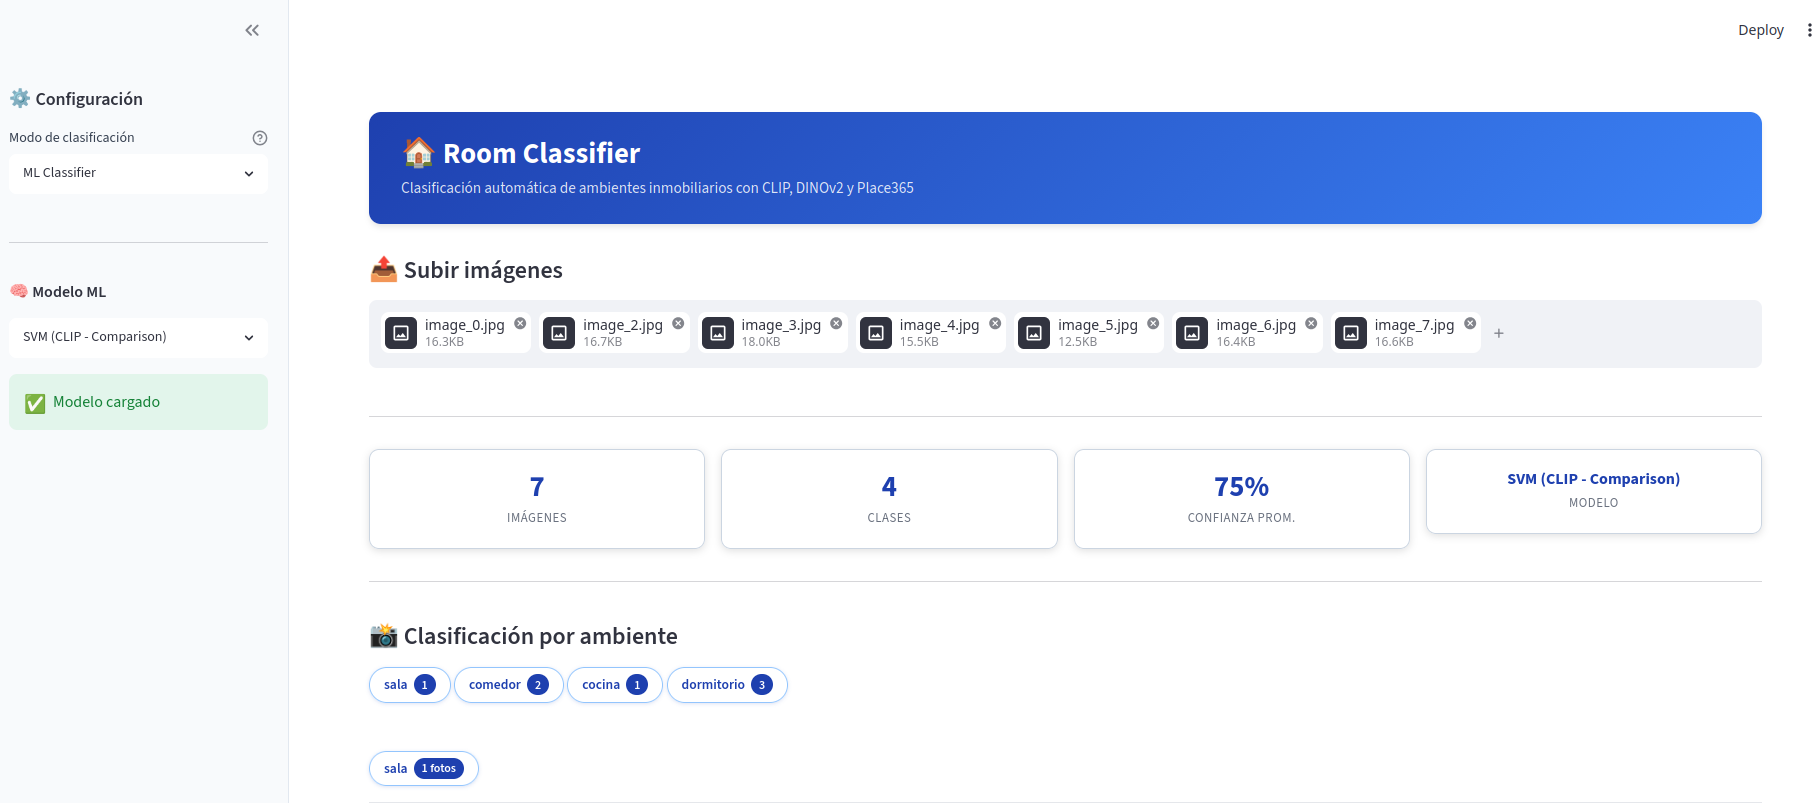
\includegraphics[width=\linewidth,height=0.60\textheight,keepaspectratio,trim=270 60 40 85,clip]{../references/mockup.png}}

\vspace{0.08cm}
{\scriptsize\color{gray} Mockup de la aplicaci\'on web: carga de im\'agenes, resumen y clasificaci\'on por ambiente.}
\end{column}
\end{columns}
\end{frame}

\section{Conclusiones}

\begin{frame}{Conclusiones Clave}
\begin{enumerate}
\item \textbf{CLIP + SVM RBF = 89.0\% F1} en 17 clases, con el mejor balance general.
\item \textbf{Embeddings congelados + SVM} ofrecen buen rendimiento sin fine-tuning pesado.
\item \textbf{Split antes del aumento} fue clave para prevenir fuga de datos.
\item \textbf{CLIP gana en 10/17 clases}; DINOv2 complementa en clases estrechas o con bajo soporte.
\end{enumerate}
\end{frame}

\begin{frame}{Trabajo Futuro}
\begin{itemize}
\item Clasificaci\'on multi-etiqueta para ambientes integrados
\item Calibraci\'on de confianza y optimizaci\'on de umbrales
\item Despliegue API REST en producci\'on
\end{itemize}
\end{frame}

\appendix
\section{Ap\'endice}

\begin{frame}{}
\centering
\Large
\textbf{\textexclamdown Gracias!}

\vspace{1cm}
\normalsize
V\'ictor Gabriel Peralta \\
gabriel.peralta.12.1998@gmail.com \\
Facultad de Ingenier\'ia, Universidad de Buenos Aires
\end{frame}

\end{document}
